\documentclass[11pt, twocolumn]{article}

\usepackage{cite}
\usepackage{graphicx}
\usepackage[english]{babel}
\usepackage{authblk}
\usepackage[T1]{fontenc}
\usepackage[utf8]{inputenc}
\usepackage{indentfirst}
\usepackage{titlesec}
\usepackage{blindtext}
\DeclareGraphicsExtensions{.png}

\titlespacing\section{0pt}{12pt plus 4pt minus 2pt}{5pt plus 2pt minus 2pt}
\titleformat{\section}
{\normalfont\large\bfseries}{\thesection}{1em}{}

\title{Hybrid Mobile Applications \\ Creating Cross-Platform Apps Using Web Technologies}
\author[1]{Andrew Zurn\\Computer Science Department\\Saint John's University\\Collegeville, MN\\awzurn@csbsju.edu}

\begin{document}
\maketitle
\tableofcontents
\begin{abstract}
Mobile applications have been in large part created using native frameworks over the course of the last few years.  Developing applications using the given tools of the device manufactures, although allowing for the creation of powerful, feature rich and smooth-acting mobile applications, has created various problems for developers looking to create applications for multiple devices.  Increased development times, multiple large codes bases, additional required expertise in development tools for each device, and rising overall costs in development has lead to what some believe is an unsustainable avenue of development. This, however, has lead to a new way of developing mobile applications, that being the "hybrid" approach, which lets developers create a single application that will port itself to many devices. ~\cite{Corral2011}  Overall, this is an area where, as hybrid technologies come closer to running as fast as natively build applications, this new paradigm for creating one application that targets many devices will see an increased popularity in use.
\end{abstract}

\section{Introduction}
Mobile development has become a large area of discourse in the computing industry, as mobile devices continue to replace traditional desktops and applications begin to be streamlined for mobile clients.  Creating mobile applications has become an industry in itself, as we are seeing the amount of mobile devices on the markets hit over nearly half a billion units worldwide ~\cite{Llamas2013}.  Therefore, creating applications for those devices has become a intriguing area for many developers. Native development has become one of the most popular avenues to create mobile applications, where developers create applications using the software development kits (SDK) provided by a device's manufacture in order to create applications that can be installed on a device, and have access to the various system and hardware features of each device.  However, this native approach towards building mobile applications, along with the proliferation of the mobile operating systems, has left developers needing to create multiple applications in order to target the large market share of mobile device users.  As can be seen in Figure 1, in order to develop to target ~90\% of the current mobile market, developers would need to build up to 4 different applications for the major operating systems, those being iOS, Android, BlackBerry, and Windows Phone. ~\cite{NetMarketShare2013}\\  

\begin{figure}[h!]
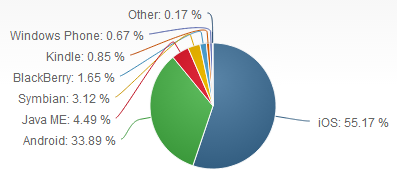
\includegraphics[scale=0.8]{mobile-market-share}
\caption{The Market Share of Mobile Devices as of Nov. 2013  ~\cite{NetMarketShare2013}}
\end{figure}

A new approach towards developing mobile applications has been set forth in the last few years, that being the 'hybrid' development solution.  Essentially, hybrid development builds an application, mainly using web technologies (HTML/CSS/JavaScript), and then in addition to using each of the various platforms SDKs, creates applications that run like a traditionally native developed app would.  There are various technical aspects to this approach, and actually two different methods this new hybrid solution uses in creating applications. Although hybrid development has its trade-offs when compared against native development, there is probable evidence that not to far into the distant future that developing mobile applications using a hybrid platform could replace the conventional method of developing natively.  In short, this new field of mobile development has various aspects, issues, and considerations to be made, which will be focused upon in the proceedings of this paper.\\

\section{Background}
Most would say mobile devices have only been around for the last 5 or so years, but they actually have their roots back to the 1990s, where the PalmOS was one of the first devices to enter the area of mobile computing. Windows even had a mobile operating system that it released in 1997. ~\cite{Dediu2011}  It was in 1998, however, that Java Micro Edition entered into the mobile race for device dominance.  Luis Corral, in his article, "Evolution of Mobile Software Development from Platform-Specific to Web-Based Multiplatform Pardigm," states that "Java 2 Micro Edition (J2ME) started opening ways to develop software for different target devices, allowing the creation of a software system in any mobile device capable to execute the Java framework." ~\cite{Corral2011}  It wasn't too much later when BlackBerry joined the mobile device industry, with the introduction of it's original devices sometime in 2002. The top current competitors, iOS and Android joined the mobile arms race a few years later, both around 2007-2008. ~\cite{Dediu2011}  As Corral points out, it wasn't soon later, after these major entities in mobile computing introduced their own platform-dependent SDKs, that "the use of J2ME decreased," and the use of these native development platforms became more popular.~\cite{Corral2011} Figure 2 offers a visual time-line of the entering of various mobile operating systems into the market up to 2013. \\

\begin{figure}[h!]
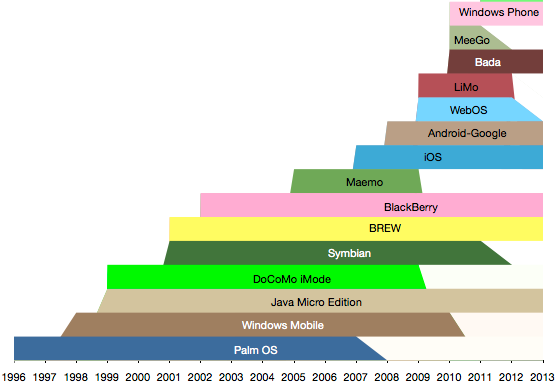
\includegraphics[scale=0.568]{mobile-proliferation}
\caption{A timeline of the major introductions into the mobile operating system market ~\cite{Dediu2011}}
\end{figure}

With the introduction of the iPhone in 2007, it was actually the intention of Steve Jobs to set out on a vision, that as Christopher Mims, states, where "web apps [would be] the future."  Apple would soon follow Google, however, by releasing their own SDK as Google did with Android in 2008.  Windows Phone was soon later, with an entrance into the market in 2010. ~\cite{Dediu2011}\\

Lately, however, a new approach has lead to a shift from the traditional development methods, and towards cross-platform development tools.  Corral explains how, "most recently, the introduction of web-based multiplatform development tools (e.g., Appcelerator Titanium, PhoneGap, or Sencha Touch) challenges current paradigms."  This new movement in development circles towards, as she goes onto proclaim, has its roots in the success of many conventional desktop applications moving towards web-based solutions, as these web-based technologies are becoming more advanced" and portable among many devices. ~\cite{Corral2011}  Olivier Le Goaer and Sacha Waltham, in their article, "Yet Another DSL for Cross-Platform Mobile Development," state that with the "lack of sustainability in software development" that they see as the problem of native development, we are now experiencing a shift towards cross-compatibility, where the slogan "write once, run everywhere," has returned to "center-stage." ~\cite{Goaer2013} In short, in the life span that we've seen mobile devices within the computing industry we've seen almost a complete life-cycle, starting with J2ME, which set out to create a framework for developers to create software for multiple target devices, to platform-specific application development tools, and now back to this new 'hybrid' solution, that leverages web technologies to create a single application that is portable to multiple target environments.\\

\subsection{Problems in Native Development}
Native development is still a widely used convention in the mobile application development industry.  However, due to the current situation where every OS on the market has their own development kit, the current environment for building applications that run natively (that is compiled, rather than interpreted ~\cite{Leroux2011}) is plagued with a handful of issues that pose serious hurdles for developers to overcome.  Developers, if they want to market towards the large market of mobile operating systems, have to replicate their applications across multiple platforms.  There are four main issues that any developer wanting to port their application will need to adjust to.  The first issue, is the increased time it will take to create multiple mobile application.  Figure 3 shows the total development time that Michael Nebeling found during his creation of multiple mobile applications.  As can be seen, about 92 hours were spent creating the iOS app, 87 hours in porting it to Android, and 72.5 hours in building the Windows Phone 7 app. ~\cite{Nebeling2013} 

\begin{figure}[h!]
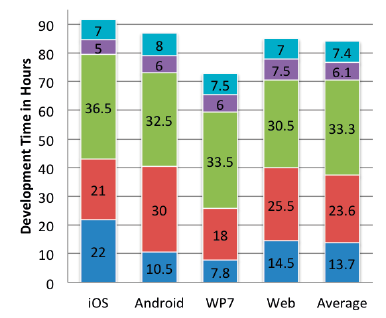
\includegraphics[scale=0.7]{dev-times}
\caption{Development times of an application on multiple devices ~\cite{Nebeling2013}}
\end{figure}

It took Nebeling over 250 hours in order to port his application to 89\% of the mobile market (referring back to Figure 1).  The next problem in creating multiple native applications is the required expertise in learning and using each different development platform.  Developers will need to learn how to use XCode and program in Objective-C if they want to create iOS apps, Eclipse and Java if they wish to build for Android, Visual Studio and a .NET language in order to create Windows Phone apps, and BlackBerry's own IDE and C/C++ in order to develop for that device.  This presents a time and effort commitment by the developer, especially if they are not familiar a the visual development environment like XCode along with the syntactically contrasting Objective-C language. We can see the difference between these two language in figures 4 and 5 below.\\

\begin{figure}[h!]
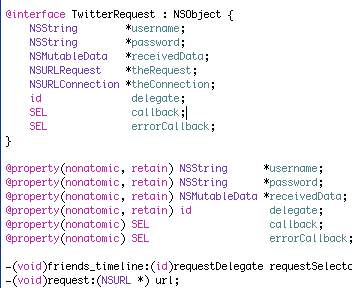
\includegraphics[scale=0.63]{obj-c-code}
\caption{Objective-C code ~\cite{Treb}}
\end{figure}

\begin{figure}[h!]
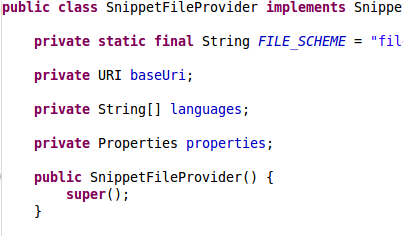
\includegraphics[scale=0.63]{java-code}
\caption{Java code ~\cite{Grott2009}}
\end{figure}

The next challenge in building native applications is the multiple codes bases that are inherent to building multiple native applications.  Large code bases means redundancy in resources, and as the multiple devices have little to no overlap in the technologies they use, almost all of the code is going to have to be replicated and written in each device's native language.  Additionally, with the massive and highly redundant code bases, the amount of time to maintain the application becomes an even larger concern the bigger these mobile applications become.\\

The final challenge is derived from the combination of the other issues that are involved with the native development method.  Increased development times, having to acquire the expertise to develop across the spectrum of available platforms, and having to create and maintain massive redundant code bases, all leads to what will likely be a huge increase in the cost that any project will see when they seek to build multiple native applications.  In short, as Corral goes on to explain, developing "a single application for each platform will eventually become redundant, expensive and unpractical." ~\cite{Corral2011}\\

\section{Hybrid Development}
Hybrid development of mobile applications, although new and largely unknown, offers many solutions to the dilemmas that face native application development.  Leveraging web technologies such as HTML, CSS, and JavaScript, a developer is able to capture the functionality of a mobile application in a common and easily understood language, and build applications to the various platforms that currently inhabit the mobile spectrum.  In this section, we'll take a look at the various approaches that hybrid application development uses to achieve its goal of porting to multiple devices, performance issues of hybrid apps, a case study using the platform {\it Appcelerator} will be given, and a comparison of the {\it Appcelerator} generated applications versus an application developed in Android will be discussed.\\

\subsection{Technical Analysis}
Hybrid mobile applications has two different models that it takes to create cross-compatible apps.  There is both a cross-compiled approach, and also an interpretative approach that both vary in how they go about creating native-like mobile apps.  Both of these models, along with a few of the platforms that employ these models will be looked at in the following sections.\\

\subsubsection{Cross-Compilation Approach}
Cross-compiled applications takes a given language that lays out the entirety of a given mobile applications, and generates the native code for each targeted platform.  Spyros Xanthopoulos and Stelios Xinogalos, in their article, "A Comparative Analysis of Cross-platform Development Approaches for Mobile Applications," examines this cross-compiled approach.  They state that these apps are "compiled just like a native app and a platform-specific version of the application is created for each target platform." ~\cite{Xanthopoulos2013}  Goaer takes a look at a platform that uses this method, called {\it Applause}.  "Applause is a DSL (domain specific language)," which is a language that has been developed specifically for this cross-compiled model, "using the Xtend technology to generate native iOS, Android, or Windows Phone 7.  That code, Java, Objective-C, C\#, or Python, is human-readable, and can be reworked before deployment." ~\cite{Goaer2013} Cross-compiled applications have access to the system and hardware features that any native application does, and also has very native-like performance. ~\cite{Xanthopoulos2013}  This approach, however, benefits more in applications that are more data-driven, as Xanthopoulous points out, where the "main functionality involves create, read, update and delete operations (CRUD) and other data-centric operations like tabular views and data entries. ~\cite{Xanthopoulos2013} \\

\subsubsection{Interpretive Approach}
The interpretive model provides, much like the cross-compiled method, a developer to build an application using a common language, and eventually deploy a native application from whatever platform they use.  Xanthopoulos again takes a look at this hybrid model, and provides some analysis into how it functions.  He states, "in interpreted apps native code is automatically generated to implement the user interface. The end users interact with platform-specific native user interface components while the application logic is implemented independently using several technologies and languages, such as Java, Ruby, XML etc." ~\cite{Xanthopoulos2013} Essentially, the interpretive app combines each platforms native SDK to build the UI elements of the app (buttons, text fields, tables, etc.), and captures the dynamic aspects of the application in a select language.  The applications is then given an interpreter that reads the code to add the dynamic features of the native application. ~\cite{Goaer2013}  One such platform, as Goaer takes a look at, is {\it Appcelerator Titanium}, which he states "precompiles JavaScript code into a set of symbols, resolved based on the targeted mobile OS (compiled .o files for iOS, .class files for Android)."  He goes onto say that included in the app is a "JavaScript interpretor," which is used to add the functions and dynamic aspects to the native-generated components.  ~\cite{Xanthopoulos2013} \\

The main difference between this model versus the cross-compiled approach is that only compiled code is packaged in addition to an included interpretor, into the end product of the interpretative platform, such as {\it Appcelerator}, while native code, that a developer can then go and edit, is generated in the cross-platform approach.  The performance of interpretive applications, however, is not as good as cross-compiled apps, as there is some overhead needed in interpreting the code that contains the dynamic aspects of the application.  Figure 6, below, offers a comparison table of the features of interpreted against cross-compiled applications.\\

\begin{figure}[h!]
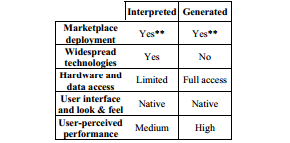
\includegraphics[scale=1.15]{int-vs-cc}
\caption{Comparison table of interpretive vs. cross-compiled mobile apps ~\cite{Xanthopoulos2013}}
\end{figure}

\begin{figure*}
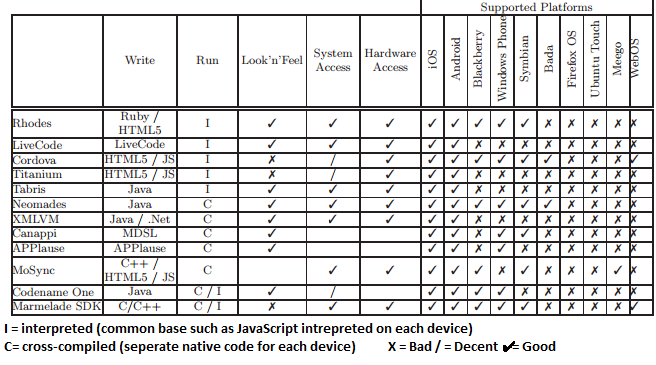
\includegraphics[width=\textwidth, height=7cm]{cross-platform-chart}
\caption{Comparison of Hybrid Development Platforms ~\cite{Goaer2013}}
\end{figure*}

Although {\it Applause} and {\it Appcelerator} are both platforms that leverage this hybrid solution, there are various other development platforms and tools existent today that allow developers the power to build a single base of code for an application, and port it to many devices.  Goaer provides a great comparative analysis of many of the platforms today, how they perform the creation of their hybrid applications, and how they comparative in different areas against each other (such as performance, look and feel, and access to the device).  A table highlighting all of this information is given in figure 7. \\

\subsubsection{Performance}
One of the largest draws towards developing native applications is how fast they run, as they are compiled into code that runs directly on the device's hardware, rather than being run through an interpreter like most web technologies are, or in our case, like {\it Appcelerator} does with its JavaScript code.  In an article that compares the mobile platform {\it PhoneGap} to a natively developed app, Ngu Phuc Huy and Do vanThanh evaluate, and also give some quantified data that compares the two apps.  In the article, they state, "PhoneGap apps cannot replace native apps because they perform slower than native apps due to the overhead from abstraction and HTML rendering in addition to the time to execute the native processes." ~\cite{Huy2012}  Brian Leroux and Andre Charland support this opinion in their article, "Mobile Application Development: Web vs. Native, stating "when interpreting code, the more there is to interpret, the longer the executing time.  Here the Web technology stack has some catching up to do.  JavaScript, for all its leaps in performance, is still slower than native counterparts. ~\cite{Leroux2011} \\

The amount of time, if, for example, in executing interpreted code at an eighth of a second versus native code executing at a sixteenth of a second, after all, probably will not matter to the average mobile user.  Huy and vanThanh provide some data in their research that depicts the amount of time a user will spend performing a task on a natively developed application, compared to how much time they spend doing the same task done in a hybrid app.  Below, in figure 8, it can be seen, that although the hybrid app does perform slower than the native app, it averages around only 2-3 seconds slower in performing the given task multiple times, which will probably be less than noticeable for a common user.\\

\begin{figure}[h]
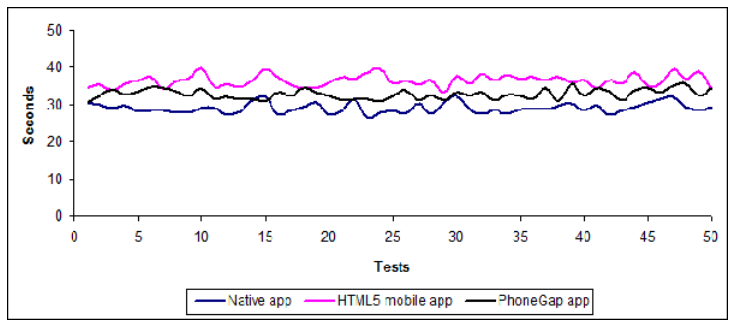
\includegraphics[scale=0.4]{huy-app-performance}
\caption{The amount of time to use the native app, HTML5 mobile app and PhoneGap app in comparison ~\cite{Huy2012}}
\end{figure}

Overall, hybrid app performance, especially in the interpretive group of developed applications, does prove to be slower in performance than their native counterparts.  Cross-compiled applications suffer less from this, as they don't actually have to do any interpreting of code (they are completely native apps).  In the end, although native apps do execute faster than hybrid-driven applications, the gap between those times in only noticeable in a few seconds when performing tasks on each platform, and as Leroux points out, as the web stack becomes faster, so will the performance of these apps, and thus the gap will decrease. ~\cite{Leroux2011}

\subsubsection{Appcelerator}
During the research done in this paper, a prototype mobile applications was also created using the hybrid platform, {\it Appcelerator Titanium}. {\it Appcelerator} is a hybrid platform that is an eclipse-based IDE and uses JavaScript as its language that will be interpreted to provide the dynamic aspects of the native-like app it creates.  It uses each platform's SDK to build out the native components of the application, then links those components to the functions and processes written in the application code.  Currently the platform can port applications to iOS, Android, BlackBerry, and Mobile Web, and will soon be supporting Windows Phone ~\cite{Appcelerator.com2012}  Below is a figure from Tim Poulsen, the Director of Training and Curriculum Development, provides some insight into how the platform functions to deploy multiple mobile applications.

\begin{figure}[h]
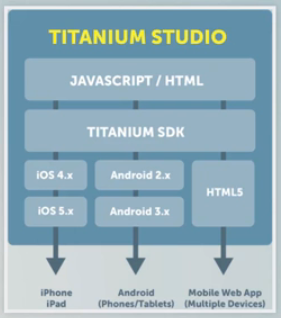
\includegraphics[scale=1]{appcelerator-flow-chart}
\caption{Flow Chart on how {\it Appcelerator} Builds Native Applications ~\cite{Poulsen2012}}
\end{figure}

As can be seen, the application is coded JavaScript/HTML, and then is passed onto the Titanium SDK, which builds the native components for the targeted platform.  {\it Appcelerator} then packages the app for that platform with a JavaScript interpreter so the native application can go back to the JavaScript/HTML and add the functional features of the application.  In the end, we have native components that are linked to the dynamic aspects of the app that is interpreted JavaScript code.\\

\subsubsection{HIPAA App Prototype}
This application was actually initially built using Eclipse on the Android platform, in order to allow for a comparison of it against the same app developed using {\it Appcelerator}.  The application that was chosen to be created is a reference course for those working in the medical industry, where every year a renewal course on HIPAA Security and Administration policies is needed to be taken.  This application offers reference material that is arranged in to chapters and sections that the user can browse to find material on different policies regarding HIPAA.\\

The Android app, even with previous development experience in Android, was difficult to develop and quite time consuming.  Android, although using Java and XML, which are both familiar languages to myself, seemed to make things overly complicated by almost forcing the developer to take into account every detail as to what the application is doing.  When developing for Android, you need to have something keep track of what is happening in the different states of the application (hidden, running, not running, etc.), and also, in my case, implement a rather complex callback system that would return a user to the previous screen (this is standardized and done for you in Appcelerator development).  Multiple objects, such as a View object, a ListContainer, and a Fragment, all had to be used to create a simple list of the chapters that the user would be able to select from. Below is a figure displaying one of the views of the final product of the Android implementation. Overall, the android application made for about a week-long development time (35-40 hours) in order to perfect the linking of chapters to sections and sections to the actual course material, and ended up being about 1000 lines of code (LOC) in length.\\

\begin{figure}[h!]
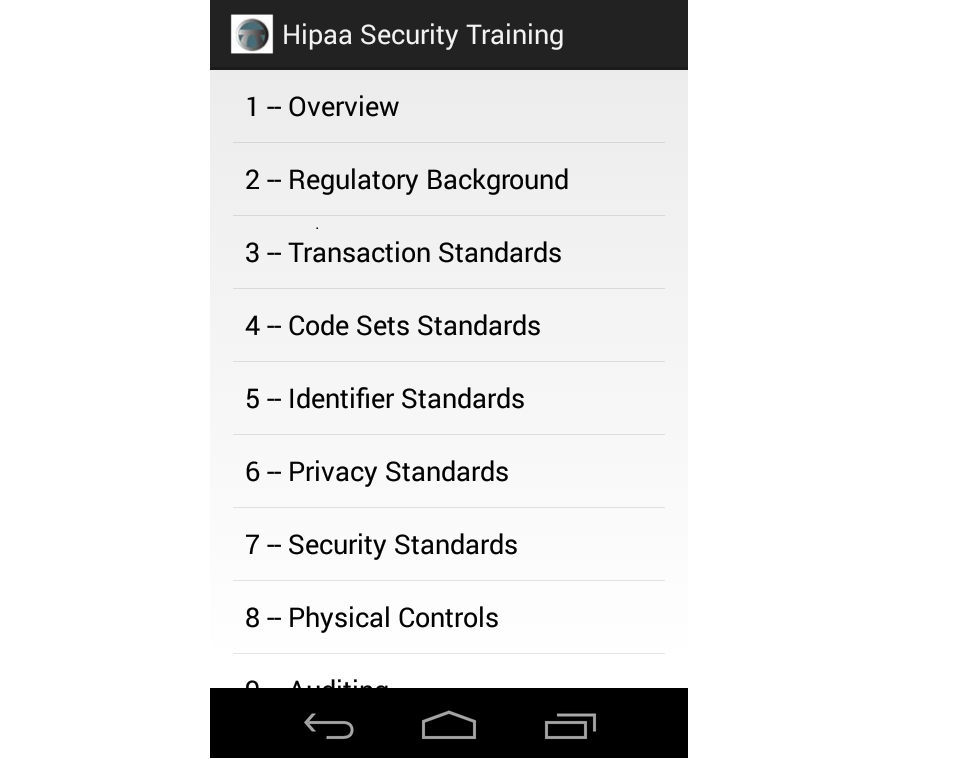
\includegraphics[scale=0.35]{android-chapter-implementation}
\caption{The Android implementation showing a list of Chapters within the course.}
\end{figure}

Developing in Appcelerator proved to be a lot less time consuming, didn't require for as much complexity and overhead to be accounted for as in the android app (no need to implement callbacks to old views), and limited the amount of needed classes to three, where as the Android app used eight different classes to implement.  The application, on the whole, took about 10 hours to develop and test, whereas the Android app took about 35-40 hours to develop.  To display a list of chapters, the data was drawn upon from a table and then told to be displayed in the view. The callback system was mostly taken care of by {\it Appcelerator}, which would keep track of the last view displayed before the current one, and then just move back to that when the back button was pressed.  When a chapter was selected, a function would be called to trigger the new view, which would find the data for that chapter from another table, and then display its sections.  Below is a figure of one of the screens of the initial prototype of the {\it Appcelerator} generated mobile app.  Overall, the implementation done in Appcelerator made for a much smoothing development process, was 410 LOC, and was significantly less complex to write, while at the same time performing all the same functions as its Android counterpart.\\

\begin{figure}[h!]
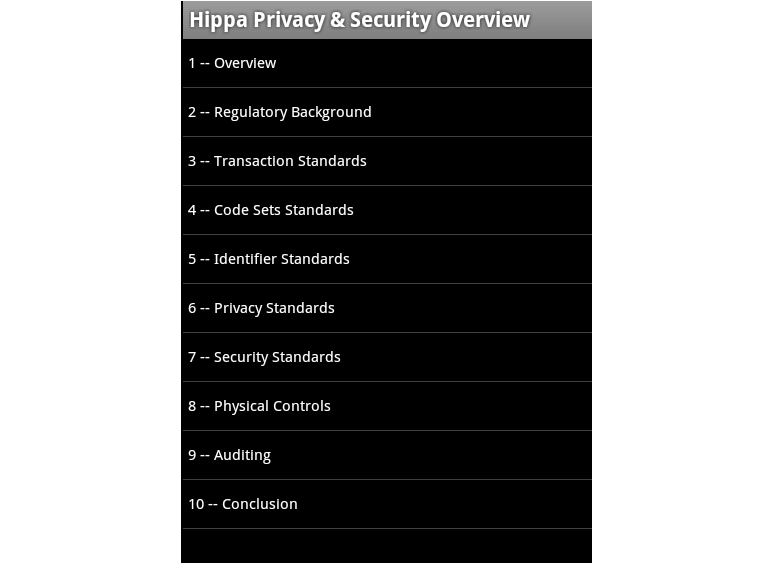
\includegraphics[scale=0.4]{appcelerator-chapter-implementation}
\caption{The Hybrid implementation showing a list of Chapters within the course.}
\end{figure}

When comparing the code of the two implementations, it can be easily seen that the {\it Appcelerator} platform delivers the tools to worry less about how something is happening, and just describe what needs to happen (6 lines of code to tell the application to move to the next view, as is seen in figure 13).  Android, on the other hand, forces the developer to setup a new Intent class, which holds the information from the previous view, state which view its going to go to next, pack the Intent object with the necessary data for the next view, and then start the next activity (figure 12).  Although this is not a terrible feature of Android, as it does give the access to explicitly describe everything that should happen, which is good for the advanced developer looking to optimize his application, it does introduce, at times, an unnecessary amount of complexity.\\

\begin{figure}[h]
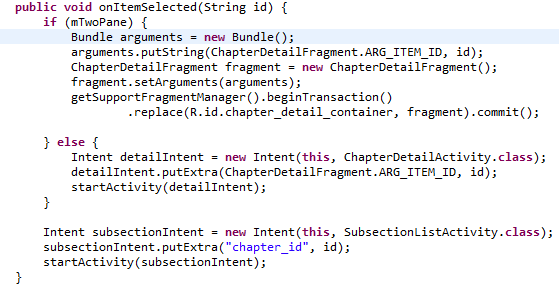
\includegraphics[scale=0.6]{android-code}
\caption{Android method to open a new view containing section data ~\cite{Poulsen2012}}
\end{figure}

\begin{figure}[h]
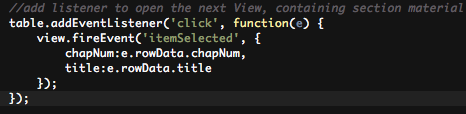
\includegraphics[scale=0.6]{appcelerator-code}
\caption{Appcelerator code to trigger a new view containing section data ~\cite{Poulsen2012}}
\end{figure}

In the end, the hybrid prototype implemented in {\it Appcelerator} proved to be the tool with the greatest advantages, and highlighted that is does indeed solve many of the problems associated with native development.  Development time of the application was drastically lower than it's native counterpart (10 hours compared to 35-40 hours). The implementation in JavaScript was fairly easier than the Android implementation in Java, showing that less required knowledge is needed to build one application that has the ability of porting to many target devices.  Less overall code was also generated, and again, having the availability of deploying one app to many devices means we don't have to have multiple seperate and highly redundant code bases for each native platform.  In the end, if we factor in all of these benefits that we find in hybrid development, with the addition that cost is going to be greatly reduced due to these considerations, hybrid development poses a great opportunity and a powerful alternative to developing mobile applications in a native framework.

\subsection{Native - Hybrid Comparison}
Hybrid mobile application development obviously shows that it is becoming a great alternative to native development tools.  There are trade-offs, however, when it comes making a decision to go with a hybrid approach versus a native approach.  For everything that hybrid apps sets out to solve in the problems that the native paradigm creates, it does stumple in one area, that being in the area of performance.\\

When discussing various matters and topic areas in any field within Computer Science, there is always a figurative tool that we can use for comparison, that being the 'better, faster, cheaper, pick two' model.  If hybrid development were to pick two of these areas, it would be better and cheaper.  Hybrid development can deliver a better overall product, in a lot cheaper fashion as the development process only has to be done once, rather than each time for each different platform a developer is targeting.  Faster, is the one area that hybrid development can not stand up to native development in, as was discussed in section 3.1.3.  This fact, however, is really not an issue, as figure 8 shows, where the actual time to use the application was only seconds slower than the native application.  In addition to this, Brian Leroux offers a few words on how insignificant this point is, as he states,

\begin{quote}
the time it takes a programmer to write comparable logic in a native compiled language on multiple devices may be worth the time penalty for execution, this will certainly also require more maintenance than one code base written in JavaScript that can be run on multiple devices.  Less code often leads to less and easier maintenance. ~\cite{Leroux2011}
\end{quote}

\begin{figure*}
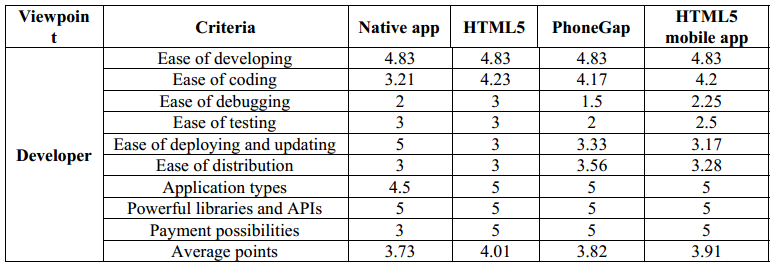
\includegraphics[width=\textwidth, height=4.5cm]{hybrid-native-compare-table}
\caption{Comparison of Native, HTML5, and Hybrid Development ~\cite{Huy2012}}
\end{figure*}

Huy and vanThanh also provide some insight and quantified data into the general aspects that hybrid and native development can be compared on.  On the average, as can be seen in figure 12 below, the hybrid application developed using {\it PhoneGap} scores both higher in the easiness of coding the application (4.17/5 versus native at 3.73/5), and also has a overall score of 3.82/5 (native development at 3.61/5). Huy offers some insight into this, as he states that

\begin{quote}
Developers prefer HTML5/PhoneGap mobile apps to the native app paradigm even though there is sufficient support to hook into a device's hardware feature for both paradigms.  The reason is that the HTML5/PhoneGap code to access a device's hardware and Web services is less verbose and complicated than native code.
\end{quote}

As was discussed in the section 3.1.5, writing the code for a hybrid application is often times easier than its native counterparts, which becomes an attraction for developers.  Being able to build an application once, and do so with a lot less effort in working with the complexities of the language it is implemented in is a significant advantage of hybrid technologies over what traditional methods of native development have provided.

In the end, as can be easily seen in figure 13, hybrid development stands up to, and offers a very similar, if not better option to development in some respects to native development.  Although performance is an issue in hybrid development, the significance of it is small and should not be undercut by the other great benefits that it offers to developers for creating mobile applications.

\begin{figure}[h]
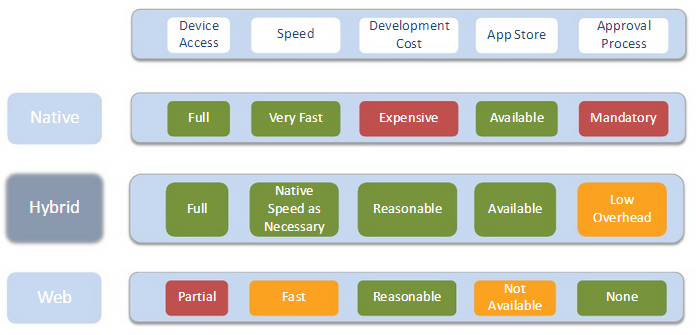
\includegraphics[scale=0.5]{ComparativeTable}
\caption{Comparative Table between Different Development Approaches} ~\cite{Kaminitz2012}
\end{figure}

\section{Future Trends}
Mobile development has almost seen a complete lifecycle of the technologies it's used, having started with mobile web apps, then moving towards platform-specific SDKs as it allows developers the options to use many of their devices powerful features, and now is starting to return to a hybrid-centric approach, that leverages web technologies where apps are built once and run on many devices.  Native apps have created a volatile development environment, where developers are plagued with issues like massively increased development time, multiple code bases, a need to acquire skills in various languages and development platforms, and overcome the costs of production when all of these are put together.  Hybrid technologies, however, have provided a solution to many of these inherent problems in native development.\\

The web stack is providing the new means to develop mobile applications, where platforms such as {\it Appcelerator} and {\it PhoneGap} are giving the developers the tools to build native-feeling and acting applications, while allowing them to write only one applications, mainly using JavaScript to do so.  This is where the continued discourse of native versus hybrid develop will take place.  As web technologies become more powerful, and the JavaScript interpreter becomes faster, these hybrid applications will become more and more attractive for those looking to develop their mobile applications.  Brian Leroux underscores this, state that although "the web technology stack has not achieved the level of performance we can attain with native code, it's getting close.  We're confident that Web technologies will become indistinguishable from native experiences." ~\cite{Leroux2011}\\

Not only is the fact that these platforms becoming more powerful over time a reason as to why hybrid development will soon to be replacing native methods, but the fact that the code used in these projects is so highly reused means developers will be able to create greater, more beautiful and feature-rich apps a lot faster than they would if the needed to focus on multiple apps at once.  Appcelerator makes the exclamation that "a single team with JavaScript experience can build an app for iOS, Android, BlackBerry, Windows, and HTML5, with up to 90\% code reuse.  The result is significantly lower cost and faster time to market."  ~\cite{Appcelerator.com2012}  Additionally, they make the point that the amount of developers that have some JavaScript/HTML experience is obviously going to be a lot more than those containing Java or iOS skills, and thus they hybrid options will be a lot more attractive than their native cousins. ~\cite{Appcelerator.com2012} In the end, it is because of not only this, that developers will no longer need to become entangled in multiple mobile environments, but also that the JavaScript engine will become faster and more indistinguishable" over the course of the next few years, thus bridging the only gap that native development has on hybrid right now, that will lead to the eventual replacement of the conventional native development methods and return full-circle to web-employed, hybrid technology platforms. ~\cite{Leroux2011}

\section{Conclusion}
Native application development, has been pretty much the only option for building feature-oriented, powerful and smooth running applications that mobile users have come to expect.  Not only are we moving into the age of mobile technology, we are also moving into the age of mobile diversity, which is driving many designers and programmers to have to build their application multiple times in order to reach the larger potions of the market.  If developers are looking to target 90\% of the mobile market, they are going to have to build their applications for Android, iOS, BlackBerry, and Windows Phone, and maintain them as these major operating systems are always seeing new releases and features being added to them on almost a monthly basis.\\

Every platform in the current native development environment has their own language and own tools that are used to create applications to run on their device. This presents a few major problems that clash with a lot of the formal ideas software engineers stand on.  One of the main problems is the fact that developers will need to redo a large part of their work, rather than being able to reuse previous code.  Furthermore, this leads to increased development times and a need to acquire the skills and knowledge to create a smooth mobile application experience.  Additionally, the amount of redundancy, and the costs needed to maintain the multiple applications are almost sure to drive any software engineer mad.\\

Hybrid mobile development seeks out to correct many of the complications that come along with native development.  Using a framework such as {\it Appcelerator}, one is able to maintain a single code base, with almost "90\% code reuse," ~\cite{Appcelerator.com2012} deploy applications to a wide range of the operating systems on the market, and leverage a very common language, JavaScript, in to simplify the development process of mobile applications and make it more accessible to developers who haven't done traditional mobile development.  Although we are now just returning to this idea of applications that would leverage web technologies in order to run on an array of devices, this concept could be drawn back upon Steve Jobs and his introduction of the iPhone. Christopher Mims of MIT states that Steve Jobs was just "a little to far ahead of the curve," in his belief that this technology would be how mobile apps would be created in the future.  Consequently, he was not far off the mark, as we are now returning to this idea that might have come from one of the world's greatest thinkers.\\

In the end, hybrid application development now poses a working solution for many of the problems we've seen with development over the last few years.  Luis Corral solidifies this point, when he exclaims that this new hybrid-based paradigm

\begin{quote}
will change the way mobile applications are developed, as this approach slims down the mobile software development process and broads its impact.  It opens the opportunity of reducing development costs and relieves the problems associated with target-specific development, such as translating from language to language, using diverse platforms or dealing with redundant efforts on coding, testing, and deployment.  Finally, it will allow developers to structure a software process for a variety of platforms, targeting their final products to a wider extent of potential customers by conducting a single development process only. ~\cite{Corral2011}
\end{quote}  

Overall, hybrid application development will likely grow and become more powerful as the main web technologies that are the driving force behind it, such as JavaScript and HTML5, become more refined and powerful in the years to come, and as more people understand that it is one of the best solutions to solve the problems that are currently within the mobile development environment today.

\bibliographystyle{plain}
\bibliography{FinalPaperBibs}

\newpage

\section{Educational Considerations}
My time and experiences both inside and outside of the classroom at Saint John's University has led to not only what I feel is a successful capstone experience, but has also deepened and made more useful the skills and knowledge that I have acquired during my undergraduate studies.  The classes that I've taken, time spent on the programming and robotics team, and the internships I've had have all built off the experiences of each other, and given me many tools that I know I will continue to use after the conclusion of my time at SJU.\\

There are various courses in particular that have provided much of the basis for what I've taken on and used through the entirety of this project.  The first of those courses would be CS162 - Data Structures.  This was the course where I truly began to understand programming and syntactic conventions, and learned to ask the questions that I needed answers to.  In addition to this, the actual material of the course made me realize the extent to which I would need to learn about the tools I was using.  Getting right to the bottom of how data structures were organized, and how to build them from the ground up provided an opportunity for me to really dig into the material of the course, and learn how these objects functioned.  It started the basis for me in which I would continue to try to fully understand the material and technologies I would use, and not just take it at the surface level.\\

The next course that I would accredit much of my success to would be CS230 - Software Development.  This course really pushed the envelope in terms of how much time I would need to put into course work and the project associated with it in order to have a rewarding experience.  I took away from this the fact that I would now need to put a lot more time and effort into every course that I took part in, in order to not only achieve a good grade, but also take away the knowledge and skills that is the objective of the course.  This was one of the courses where the outcome was also deepened in part by this current project, as I learned more about research and how that is conducted, and how it can and should often times be done on anything that you are working on.\\

The final course that I would relate to this in the terms that it provided for some of the basis of this courses' success, is CS330 - Software Engineering.  It was this course that first introduced me to Android, Eclipse, and GitHub which previous to this I had never used before.  Moreover, it was the way that these environments were introduced, with little to no help outside of resources online, that I benefited the most from.  Having to find my answers to the problems I encountered with Android and GitHub only deepened my skills of online research and figuring out how to ask the questions that would return the best results.  Additionally, having the background in Android from this course was more or less the foundation for the interest that I procured in mobile development that let to the eventual topic of the research project.  Learning how to use Eclipse for the first time also gave me the confidence to dive into new tools and platforms, and search out the expertise of those that already had experience using those tools, as my teammates did have when using Eclipse.  I've come to realize this more and respect the teaching of that course through my progress in this project. Simply picking up new technologies and struggling through them in order to learn them through and through has helped me in this course, having picked up this new hybrid platform of creating mobile applications, and is something I will continue to use and prosper from outside of school.\\

I feel that I've also benefited from my years spend on both the programming contest and robotics contest teams.  This provided a new opportunity to work with students that were older and more knowledgeable at the time than I was.  I was inspired by these people to work harder, and try to learn as much stuff from that, usually on topics that weren't discussed inside the classroom, as I could.  Furthermore, these two activities provided a means for thinking that usually wasn't done in the classroom or on homework.  They pushed me to think on my feet and try to produce quick solutions when under time restrictions.  Although this isn't directly a beneficial feature of the activities, that is I think it is still better to take time to research and full understand something before tackling the problem, it did push again, much like the other three courses did, to understand the tools I had available to me, and find creative ways to solve a problem using them.  Overall, I would have to say I became a better programmer and creative thinker from not only the courses that I've discussed above, but also in large part from these two activities.\\

I would also like to benefit my internship during the summer of 2013 at Thomson Reuters for learning how to not only become a better programmer, but learn how to more effectively interact with people.  I went into this summer not knowing what I would be working on, and was again presented with tools and a language that I would have to learn from the ground up, those being Java Server Faces (JSF), and JavaScript.  Having to learn both of these languages only reinforced my skills in picking up something new and learning how to use it, but learning JavaScript also presented the building blocks that I would later use during this project to create my cross-platform mobile application.  The other benefit that I took away from Thomson Reuters was how to interact with individuals and pull my own weight on a team.  Although I've had plenty of group experiences in the past, I would not say they were on the magnitude of the experience it is to be on when working in an enterprise.  I learned to become an expert in my area of the software development framework, learned how to answer other peoples' questions, and also learned how to seek out and ask questions of the right people.  Overall, not only did my skills as a programmer become more substantial during my time at Thomson, which helped me during this project in respects to knowing and using JavaScript, but I also learned the soft skills of working within a business and working on a programming team, of which I will go on and continue to use in the coming years as I enter into the computing industry.\\

In the end, what I would say that I've used the most in this project, of which I've taken away from my previous experiences to this is the way to research, answer my own questions, and use and become familiar with new tools that I have little to no working knowledge of.  My courses in the Computer Science major at Saint John's has allowed me to become familiar with the concepts of programming and showed me how much work would need to go into something to make it successful.  Taking these into consideration with my courses like CS330, my internships, and this current course, I've been able to pick up the {\it Appcelerator} platform, learn a lot of the functionality of it, and produce a successful prototype using it.  Overall, this project, the research I've put into it and the skills I've taken out of it make me appreciate the education that I've attained from my time as a Computer Science major, and is something I will be able to build on further as I move into the work world and eventually onto the possibility of further education.\\

\end{document}